\begin{blocksection}
\question Write a function, \lstinline$replace_x$ that takes in a tree, \lstinline$t$, and returns a new tree with all
labels \lstinline$x$ replaced with 0.

For example, if we called \lstinline$replace_x(t, 2)$ on the following tree:

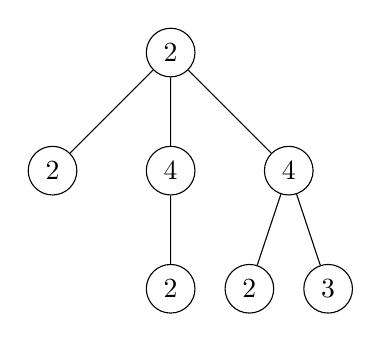
\begin{tikzpicture}[scale=1, transform shape]
\tikzstyle{level 2}=[sibling distance=10mm]
    \node [circle, draw] (z){$2$}
        child {node [circle, draw] (a) {$2$}}
        child {node [circle, draw] (d) {$4$}
            child {node [circle, draw] (g) {$2$}}
        }
        child {node [circle, draw] (b) {$4$}
            child {node [circle, draw] (e) {$2$}}
            child {node [circle, draw] (f) {$3$}}
        };
\end{tikzpicture}

We would expect it to return

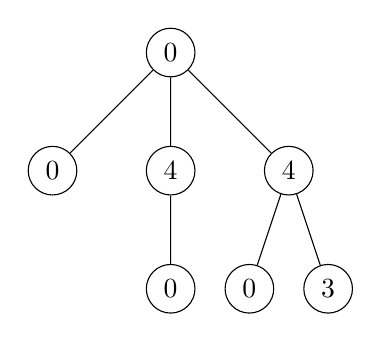
\begin{tikzpicture}[scale=1, transform shape]
\tikzstyle{level 2}=[sibling distance=10mm]
    \node [circle, draw] (z){$0$}
        child {node [circle, draw] (a) {$0$}}
        child {node [circle, draw] (d) {$4$}
            child {node [circle, draw] (g) {$0$}}
        }
        child {node [circle, draw] (b) {$4$}
            child {node [circle, draw] (e) {$0$}}
            child {node [circle, draw] (f) {$3$}}
        };
\end{tikzpicture}

\begin{lstlisting}
def replace_x(t, x):
    """
    >>> t = tree(2, [tree(1), tree(2)])
    >>> replace_x(t, 2)
    tree(0, [tree(1), tree(0)])
    """
    new_branches = []
    for _______ in ____________________________:

        new_branches._____________________________

    if ________________________________________:

        return ________________________________

    return ________________________________
\end{lstlisting}
\end{blocksection}

\begin{blocksection}
\begin{solution}
\begin{lstlisting}
def replace_x(t, x):
    new_branches = []
    for b in branches(t):
        new_branches.append(replace_x(b, x))
    if label(t) == x:
        return tree(0, new_branches)
    return tree(label(t), new_branches)
\end{lstlisting}

An alternate solution using list comprehensions is as follows:

\begin{lstlisting}
def replace_x(t, x):
   new_branches = [replace_x(b, x) for b in branches(t)]
   if label(t) == x:
        return tree(0, new_branches)
   return tree(label(t), new_branches)
\end{lstlisting}

Here, we construct and return a new tree. First, we construct a new list of branches where each branch is the same
as the previous branch but all occurrences of x have been replaced with 0 as per our recursive function. 
The if statement guarantees that if our root node's label is an occurence of x, we replace the subtree we're on starting at its root --  
keeping all else before it the same while replacing the specific subtree's root node label to be zero.
\newline
We do not need a base case here, as if we are at a leaf, the list
comprehension we use to create the new branches will evaluate to an 
empty list. Then we will either return \lstinline$tree(0, [])$ or
\lstinline$tree(label(t), [])$ as appropriate. 
\end{solution}
\end{blocksection}


\begin{guide}
	\begin{blocksection}
	\textbf{Teaching Tips}
	\begin{itemize}
			\item Draw out a tree and ask them to play out the algorithm
			\begin{itemize}
	                \item If you were a computer, how would you replace all the \lstinline{x}'s? (Answer: check the value of the current tree, then each of the branches)
                    \item If they're struggling with playing out the algorithm, make sure to draw out how recursion would work in these cases.
	                \item Can we somehow “simplify” all of this repeated work? (A/N: This simplification begs for list comprehensions to be used. The list comprehension isn't intuitive so have them first work through the for loop skeleton code.)
            \end{itemize}
		\item Make sure they respect abstraction barriers 
            \begin{itemize}
                \item If there isn't a \lstinline{set_value} function, how can we return a tree with an updated value? (Answer: create a new tree with \lstinline{0} and the new branches)
                \item Another way to phrase this: What is the only way in which we can change values within the Tree ADT?
            \end{itemize}
		\item Warn them against trying to evaluate branches
            \begin{itemize}
                \item What is the simplest replacement we can do?
                \item How can we delegate branch replacements to recursive calls?
            \end{itemize}
            \item If we have multiple branches, how do we make the recursive call on each branch? (Answer: a for loop)
            \begin{itemize}
                \item What happens in the for loop if there aren’t any branches? (Answer: nothing)
                \item This is why we don’t need an explicit base case (ex. if len(branches) == 0)
            \end{itemize}
	\end{itemize}
	\end{blocksection}
\end{guide}

